% Options for packages loaded elsewhere
\PassOptionsToPackage{unicode}{hyperref}
\PassOptionsToPackage{hyphens}{url}
\PassOptionsToPackage{dvipsnames,svgnames,x11names}{xcolor}
%
\documentclass[
]{article}
\title{Relevant NBA Stats from 2020-2021 Season}
\author{Eduardo Salvador}
\date{May 4, 2022}

\usepackage{amsmath,amssymb}
\usepackage{lmodern}
\usepackage{iftex}
\ifPDFTeX
  \usepackage[T1]{fontenc}
  \usepackage[utf8]{inputenc}
  \usepackage{textcomp} % provide euro and other symbols
\else % if luatex or xetex
  \usepackage{unicode-math}
  \defaultfontfeatures{Scale=MatchLowercase}
  \defaultfontfeatures[\rmfamily]{Ligatures=TeX,Scale=1}
\fi
% Use upquote if available, for straight quotes in verbatim environments
\IfFileExists{upquote.sty}{\usepackage{upquote}}{}
\IfFileExists{microtype.sty}{% use microtype if available
  \usepackage[]{microtype}
  \UseMicrotypeSet[protrusion]{basicmath} % disable protrusion for tt fonts
}{}
\makeatletter
\@ifundefined{KOMAClassName}{% if non-KOMA class
  \IfFileExists{parskip.sty}{%
    \usepackage{parskip}
  }{% else
    \setlength{\parindent}{0pt}
    \setlength{\parskip}{6pt plus 2pt minus 1pt}}
}{% if KOMA class
  \KOMAoptions{parskip=half}}
\makeatother
\usepackage{xcolor}
\IfFileExists{xurl.sty}{\usepackage{xurl}}{} % add URL line breaks if available
\IfFileExists{bookmark.sty}{\usepackage{bookmark}}{\usepackage{hyperref}}
\hypersetup{
  pdftitle={Relevant NBA Stats from 2020-2021 Season},
  pdfauthor={Eduardo Salvador},
  colorlinks=true,
  linkcolor={Maroon},
  filecolor={Maroon},
  citecolor={Blue},
  urlcolor={blue},
  pdfcreator={LaTeX via pandoc}}
\urlstyle{same} % disable monospaced font for URLs
\usepackage[margin = 0.5in]{geometry}
\usepackage{graphicx}
\makeatletter
\def\maxwidth{\ifdim\Gin@nat@width>\linewidth\linewidth\else\Gin@nat@width\fi}
\def\maxheight{\ifdim\Gin@nat@height>\textheight\textheight\else\Gin@nat@height\fi}
\makeatother
% Scale images if necessary, so that they will not overflow the page
% margins by default, and it is still possible to overwrite the defaults
% using explicit options in \includegraphics[width, height, ...]{}
\setkeys{Gin}{width=\maxwidth,height=\maxheight,keepaspectratio}
% Set default figure placement to htbp
\makeatletter
\def\fps@figure{htbp}
\makeatother
\setlength{\emergencystretch}{3em} % prevent overfull lines
\providecommand{\tightlist}{%
  \setlength{\itemsep}{0pt}\setlength{\parskip}{0pt}}
\setcounter{secnumdepth}{5}
\usepackage{booktabs}
\usepackage{longtable}
\usepackage{array}
\usepackage{multirow}
\usepackage{wrapfig}
\usepackage{float}
\usepackage{colortbl}
\usepackage{pdflscape}
\usepackage{tabu}
\usepackage{threeparttable}
\usepackage{threeparttablex}
\usepackage[normalem]{ulem}
\usepackage{makecell}
\usepackage{xcolor}
\ifLuaTeX
  \usepackage{selnolig}  % disable illegal ligatures
\fi

\begin{document}
\maketitle

\clearpage

\hypertarget{introduction}{%
\section{Introduction}\label{introduction}}

This project is to be used as a way to research each player's position
to find a correlation between the data of the 2020-2021 NBA season to
see how each position in the NBA has changed from the traditional
playstyle. I wanted to be able to look at trends in the data that
suggest which position has the most and least point conversion whether
it be 3pt or 2pt and what position has on average the youngest and
oldest players. As well as answering the questions as to which NBA team
has scored the most amount of points on average and the least amount of
points on average during this season. Be aware to not use this model for
any type of sports betting since, all models are wrong, only some are
useful.

\vspace{.2in}
\hrule
\vspace{.2in}

\hypertarget{description-of-the-data}{%
\section{Description of the Data}\label{description-of-the-data}}

\begin{enumerate}
\def\labelenumi{\arabic{enumi}.}
\tightlist
\item
  I got the data from Kaggle. The link I used was:
  \url{https://www.kaggle.com/datasets/umutalpaydn/nba-20202021-season-player-stats}
\item
  This data frame has all the NBA players from 2020 and 2021
\item
  Content: 1.Per Game Stats: Basically dividing every individual stats
  by the played game . 2.Per 36 Minute Stats: In order to calculate
  per-36 minute stats, you divide 36 by the number of minutes the player
  actually played, then take that number and multiply all of the
  player's stats by it. 3.Advanced Stats: These are more focused on the
  players direct effect on winning the games or scoring a point. For
  example a key tenet for many modern basketball analysts is that
  basketball is best evaluated at the level of possessions. During a
  single game, both teams have approximately the same number of
  possessions, because they alternate possession. (A team can have
  slightly more if it begins and ends a quarter or half with
  possession.) However, over the course of the season, teams play at
  very different paces, which can dramatically color their points scored
  and points allowed per game. Therefore, these analysts favor use of
  points scored per 100 possessions (offensive rating) and points
  allowed per 100 possessions (defensive rating).
\end{enumerate}

I choose to analyze the data from the NBA 2020-2021 season since I am a
big basketball fanatic and this season was the first season I got into
NBA fantasy which for those reading who don't know is getting together
with friends to draft specific players and follow them through the whole
season while playing every single week against one of your friend's
teams and the one who has the best team wins. This also involves
constantly looking at the roster since various players suffer from
injuries as well as making sure the active players in your roster play
that week. I became a big fan of this but, unfortunately, since it was
my first time playing I did really poorly so, I want to analyze this
dataset to find the key positions I should be focusing on drafting.

\vspace{.2in}

\hrule
\vspace{.2in}

\hypertarget{methods}{%
\section{Methods}\label{methods}}

To answer the questions from the Introduction which are listed below the
following statistical methods were used to solve them:

\begin{enumerate}
\def\labelenumi{\arabic{enumi}.}
\tightlist
\item
  What position has on average the youngest and oldest players?
\end{enumerate}

For the first question, the statistical method used was multiple
boxplots to showcase each position on the x-axis and age in years on the
y-axis. This will show not only the mean age of each position but also
the distribution of numerical data and skewness by displaying this data
quartiles.

\begin{enumerate}
\def\labelenumi{\arabic{enumi}.}
\setcounter{enumi}{1}
\tightlist
\item
  Which position has the most and least point conversion where it be 3pt
  or 2pt?
\end{enumerate}

For the second question, the statistical method used was a combination
between linear regression and scatterplot to see the correlation between
the 3 pt and 2 pt attempts with the actual points scored between all the
different positions. The scatterplot helps visualize the disparities
between all the data points between all the different positions and the
linear regression helps identify the most and least point conversion
based on the slope of each line.

\begin{enumerate}
\def\labelenumi{\arabic{enumi}.}
\setcounter{enumi}{2}
\tightlist
\item
  Which NBA team has the most and least amount of points scored on
  average?
\end{enumerate}

For the third question, the statistical method used was to create a
histogram that has the Teams in the x value and the number of Points on
average scored on the y value. With this, it will be easily identified
which team has scored the most and least points on average for the
2020-2021 season.

\vspace{.2in}
\hrule
\vspace{.2in}

\hypertarget{results-and-discussion}{%
\section{Results and Discussion}\label{results-and-discussion}}

Multiple boxplot

In an initial investigation, I wanted to know the average player's age
based on their position to see if there is a correlation between player
position and the amount of experience. Based on the results, the graph
shows that the center position in the NBA on average has the oldest
players which makes sense since the center position's most important
attribute is the height of a player and it is really difficult to find
tall younger players. The graph also shows the youngest position is the
point guard and the role of small forward and power forward players.
This also makes sense since for this kind of position the most important
attribute is athleticism and strength in which young players may have
the advantage as compared to older players because age does affect this.

\begin{center}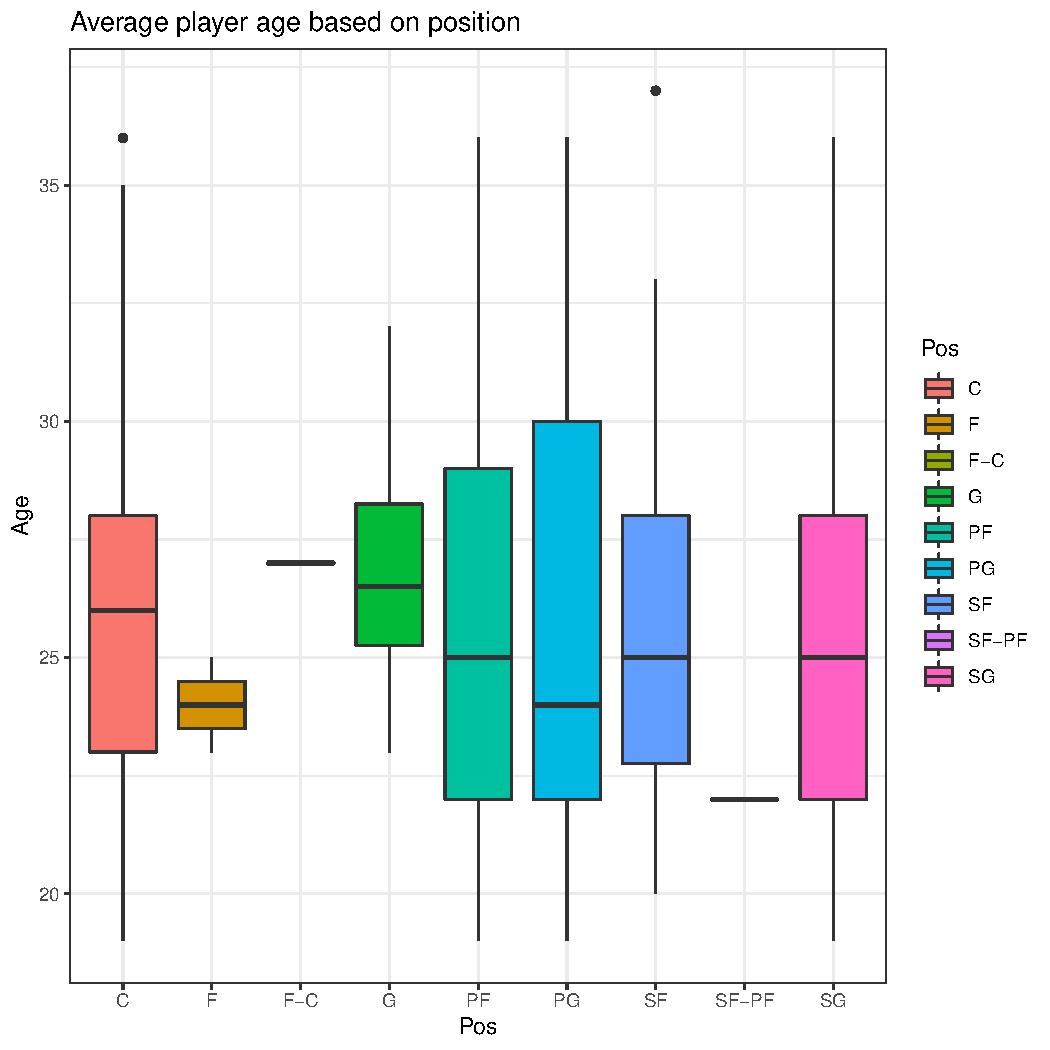
\includegraphics{./figures/unnamed-chunk-2-1} \end{center}

\begin{verbatim}
[1] 25.62374
\end{verbatim}

Linear Regression + Scatterplot

I wanted to see if there was a correlation between 3 pt attempts, 2 pt
attempts, and the number of points scored per position in the NBA. The
results from this graph suggest that on average the Shooting guard has
the highest percent 3 pt conversion out of all the positions which makes
sense since their usual role in the team is to be able to score points
from outside the box. Even so, it is interesting to see the position
with the most attempts and lowest conversion rate from 3 pt is Guard as
whereas I thought it was going to be the Center position. This is seen
in the first graph since even tho the center position is the lowest line
out of all the lines, the guard has a negative slope suggesting they are
unreliable when it comes to 3 pt scored.

The results from the 2 pt attempts and the number of points scored per
position were different which is expected. The most reliable position at
scoring 2 pts is based on the graph the Guard position which was
surprising after seeing the results of the last graph. The least
reliable position at scoring 2 pts is the shooting guard which we can
see in the graph since it has the lowest slope which was also really
surprising but, makes sense since their usual role is to hit those
3-pointers.

\begin{center}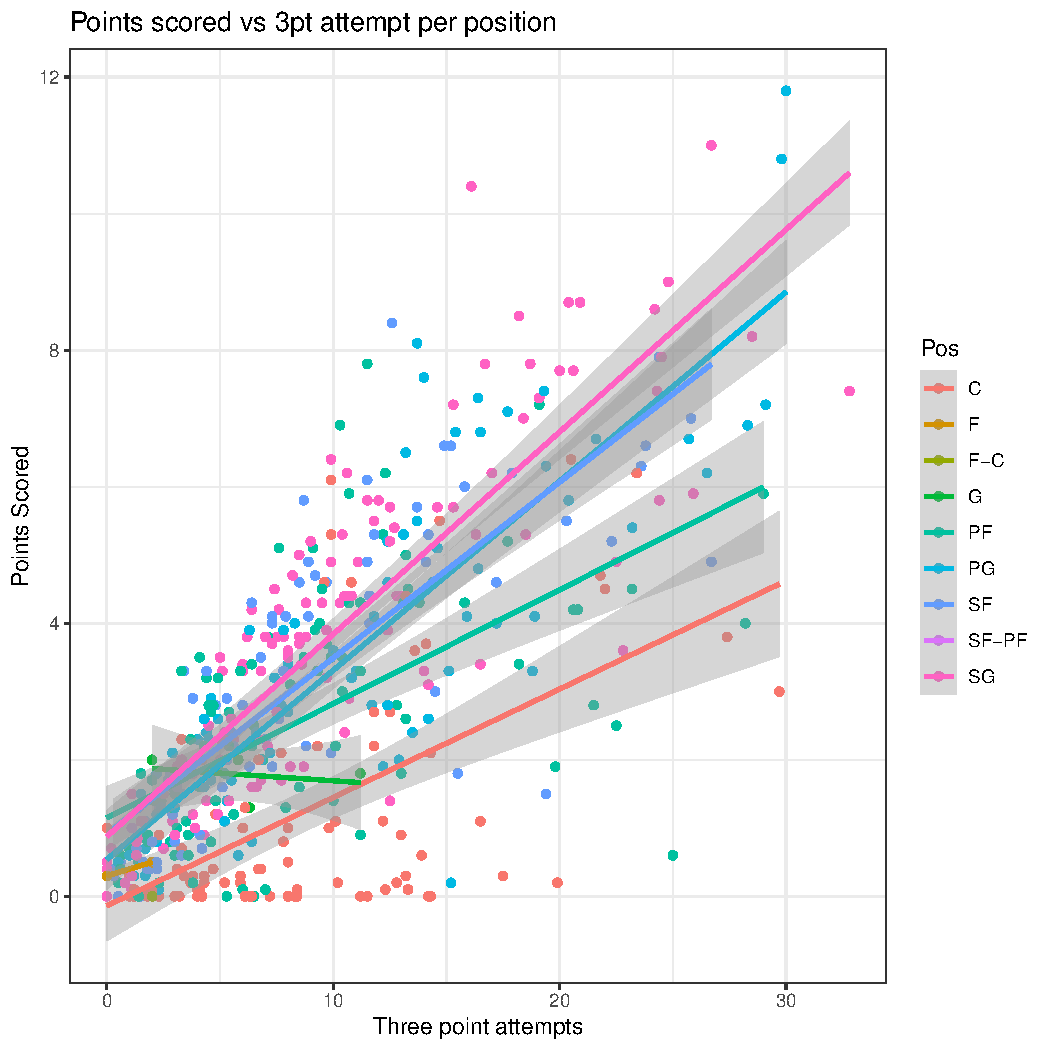
\includegraphics{./figures/unnamed-chunk-3-1} \end{center}

\begin{center}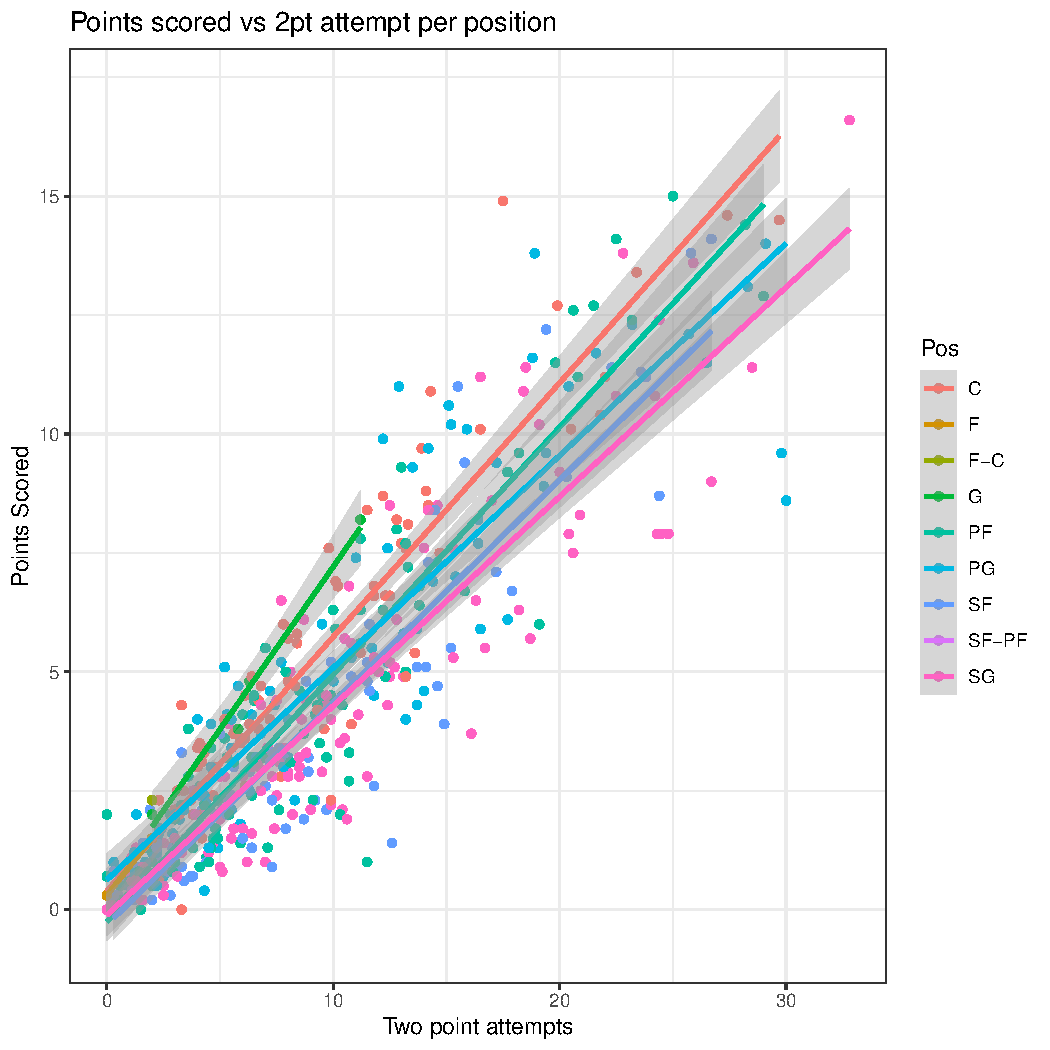
\includegraphics{./figures/unnamed-chunk-3-2} \end{center}

Histogram+Scatterplot

I wanted to see the relationship between 2-point attempts, 3-point
attempts, and the amount of points players average. The results for this
graph are interesting since the histogram suggests that players do
attempt more 2 pts than 3 pts but the scatterplot suggests that players
who attempt more 3pt do score more points at the end.

\begin{verbatim}
             Player Pos Age  Tm  G GS   MP  FG  FGA   FG. X3P X3PA  X3P. X2P
1  Precious Achiuwa  PF  21 MIA 28  2 14.6 2.6  4.4 0.590 0.0  0.0 0.000 2.6
2      Jaylen Adams  PG  24 MIL  6  0  2.8 0.2  1.3 0.125 0.0  0.3 0.000 0.2
3      Steven Adams   C  27 NOP 27 27 28.1 3.5  5.8 0.603 0.0  0.0 0.000 3.5
4       Bam Adebayo   C  23 MIA 26 26 33.6 7.4 12.9 0.573 0.1  0.2 0.400 7.3
5 LaMarcus Aldridge   C  35 SAS 18 18 26.7 5.9 12.5 0.476 1.3  3.7 0.358 4.6
6 Ty-Shon Alexander  SG  22 PHO  3  0  2.7 0.0  1.0 0.000 0.0  0.3 0.000 0.0
  X2PA  X2P.  eFG.  FT FTA   FT. ORB DRB TRB AST STL BLK TOV  PF  PTS
1  4.4 0.590 0.590 1.3 2.4 0.561 1.3 2.7 4.0 0.6 0.4 0.5 1.0 1.9  6.5
2  1.0 0.167 0.125 0.0 0.0 0.000 0.0 0.5 0.5 0.3 0.0 0.0 0.0 0.2  0.3
3  5.7 0.606 0.603 1.1 2.3 0.468 4.3 4.6 8.9 2.1 1.0 0.6 1.7 1.9  8.0
4 12.7 0.576 0.576 5.1 6.0 0.841 1.9 7.3 9.2 5.3 1.0 1.0 3.0 2.6 19.9
5  8.8 0.525 0.529 0.9 1.2 0.762 0.8 3.5 4.3 1.9 0.4 0.9 0.9 1.5 14.1
6  0.7 0.000 0.000 0.0 0.0 0.000 0.0 0.3 0.3 0.3 0.0 0.0 0.0 0.3  0.0
\end{verbatim}

\begin{center}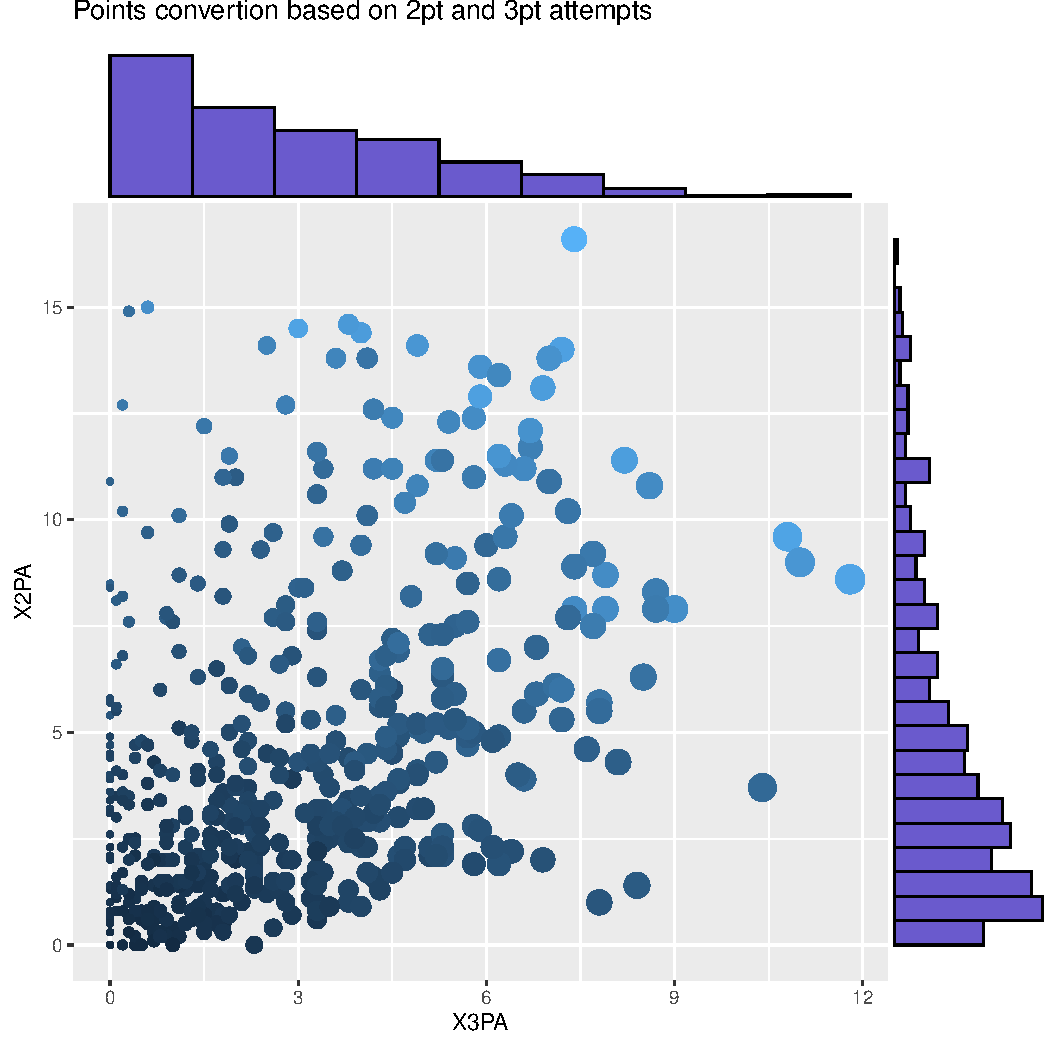
\includegraphics{./figures/unnamed-chunk-4-1} \end{center}

Histogram

The histograms show the number of points on average scored by each team
in the 2020-2021 NBA season. The result shows that the team which scored
the most points is Brooklyn Nets and the team that least scored points
on average was TOT which in this dataset means players who played for
multiple teams during the allotted season. So the true least scored
point team during the allotted season was unfortunately Los Angeles
Lakers (my team). These results surprised me since they did not do so
bad compared to this new season since they finished 10th out of all the
teams with the most amount of wins. It makes sense since most of that
season one of its best players was injured for almost every single game.

\begin{center}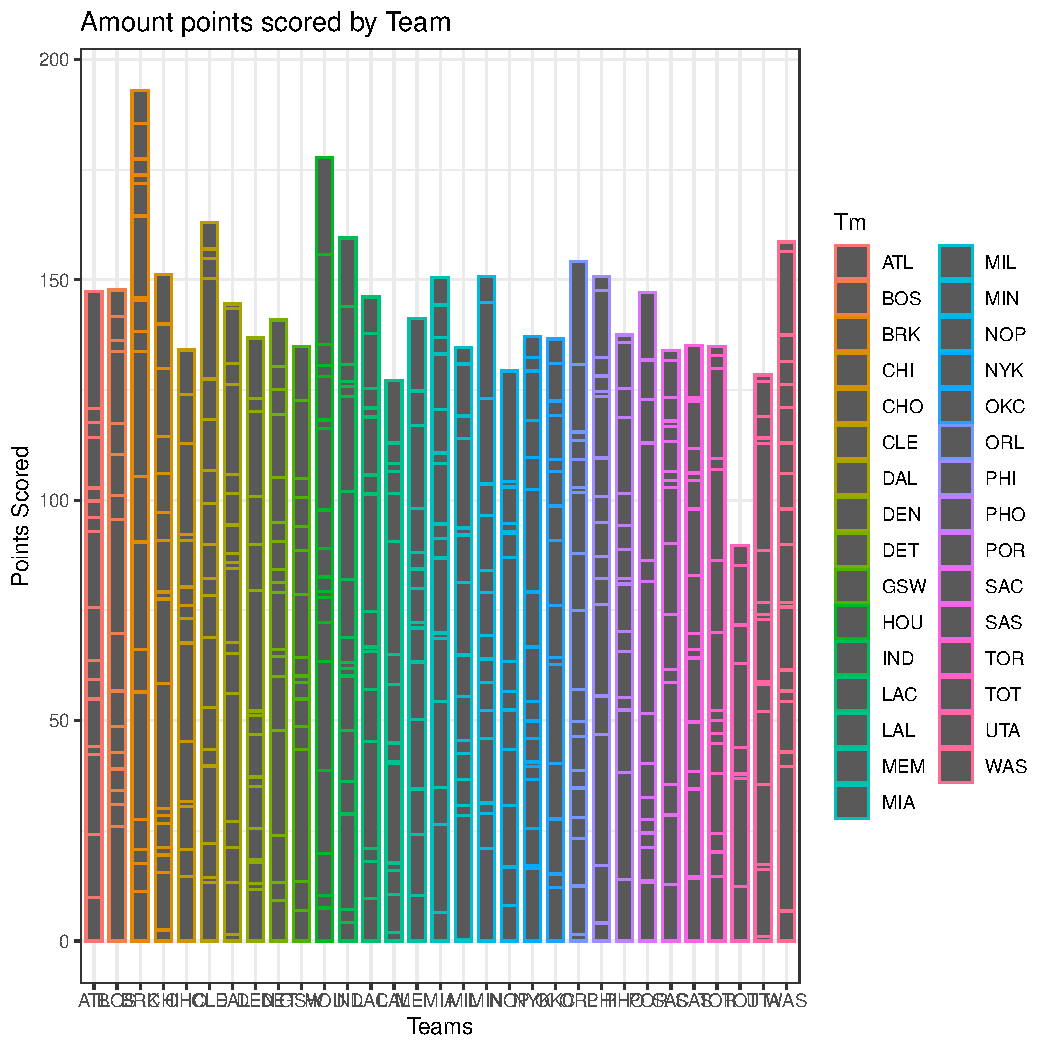
\includegraphics{./figures/unnamed-chunk-5-1} \end{center}

\vspace{.2in}
\hrule
\vspace{.2in}

\hypertarget{conclusions}{%
\section{Conclusions}\label{conclusions}}

This project was a lot of fun to do since it was open-ended as to we
decide what we wanted to look for in a dataset that had to meet certain
length requirements. The results from this project were eye-opening for
me since I didn't expect most of them. Beginning with the average age by
position, where the point guard has the most versatile age range and the
players who play Forward and Center on average are the oldest were as I
expected the Center position to be the oldest. This result made me
realize that age is just a number and that players are either good at
taking care of their body nowadays or that by changing their playstyle
they can keep being in the NBA since the Point Guard position is one
where players need to be either athletic or intelligent since they bring
the ball up the court.

Another eye-opening result came with the second and third graphs where I
didn't expect to see the guard being the least efficient at 3 pt but
most efficient at 2 pt range. Similarly, with the shooting guard, I did
expect him to be the most efficient at 3 pt but not, the least efficient
at 2 pt range. This tells me that for me to build the most efficient
draft I have to be careful which player I have to pick for these
positions since it is essential to the team.

The histogram + scatterplot graph results were also unexpected in which
it implies that the players who attempt more 3 pts end up scoring more
points than the players who attempt more 2 pts on average. It makes
sense since the game NBA has been moving towards a more 3pt game thanks
to data analytics and it shows the efficiency through this cool graph.
This finding made me realize that I need to find for my next draft
players who attempt more 3pt than average to be able to have the best
team possible just, not in the guard position seen in the results of
earlier graphs.

The last graph was something I didn't expect. As a Lakers fan, it is
hurtful to see that my team scored on average the least amount of points
out of all the teams and that the Brooklyn Nets were the opposite. I
will strongly consider this when drafting next season since, I do tend
to bias Lakers players thinking they are the best, which by looking at
the results is not the truth anymore.

\vspace{.2in}
\hrule
\vspace{.2in}

\hypertarget{appendix}{%
\section{Appendix}\label{appendix}}

\#\#Graph 1

library(ggplot2)

library(tidyverse)

library(dplyr)

library(olsrr)

library(pander)

\#Reading the file

dfadplayers\textless-read.csv(``/Users/eduardosalvador/Desktop/FINAL~Spring~Semester~2021/CMDA~/Assignments/Project~1/archive/nba2021\_advanced.csv'',header
= T)

dfpergame\textless-read.csv(``/Users/eduardosalvador/Desktop/FINAL~Spring~Semester~2021/CMDA~/Assignments/Project~1/archive/nba2021\_per\_game.csv'',header
= T)

ggplot(dfadplayers,aes(x=Pos,y=Age,fill=Pos))+theme\_bw()+geom\_boxplot()+ggtitle(``Average
player age based on position'')

mean(dfadplayers\$Age)

\#\#Graph 2

\#Created a linear regression + Scatterplot

ggplot(dfpergame,aes(x=PTS,y=X3PA,color=Pos))+theme\_bw()+ggtitle(``Number
of points per position based on field goal attemps'')+geom\_point() +
labs(x = ``Three point attempts'', y = ``Points Scored'', title =
``Points scored vs 3pt attempt per position'')+geom\_smooth(method =
``glm'')

ggplot(dfpergame,aes(x=PTS,y=X2PA,color=Pos))+theme\_bw()+ggtitle(``Number
of points per position based on field goal attemps'')+geom\_point() +
labs(x = ``Two point attempts'', y = ``Points Scored'', title = ``Points
scored vs 2pt attempt per position'') +geom\_smooth(method = ``glm'')

\#\#Graph 3

library(ggplot2)

library(ggExtra)

\#\#Looking at the top 5 rows of data regarding the dfpergame

head(dfpergame)

\#\#classic plot :

p \textless- ggplot(dfpergame, aes(x=PTS, y=X2PA, color=X3PA,
size=X3PA)) + geom\_point() +
theme(legend.position=``none'')+ggtitle(``Pts based on 2 pt and 3 pt
attempts average per game'')

\#\#Custom marginal plots:

p2 \textless- ggMarginal(p, type=``histogram'', fill = ``slateblue'',
xparams = list( bins=10))

p2

\#\#Graph 4

\#Created ggplot histogram

ggplot(dfpergame,aes(x=Tm,y=PTS,color=Tm))+geom\_bar(stat =
``identity'',width = .7)+theme\_bw()+labs(title = ``Amount points scored
by Team'')+xlab(``Teams'')+ylab(``Points Scored'')

\vspace{.2in}
\hrule
\vspace{.2in}

\clearpage

\clearpage

```

\end{document}
